\documentclass{report}
\usepackage[total={6.5in,9in}]{geometry}

\usepackage[fleqn]{amsmath}
\usepackage{amssymb}
\usepackage{titlesec}
\usepackage{fontspec}
\usepackage{color}
\usepackage{pxfonts}
\usepackage{cancel}
\usepackage{multicol}
\usepackage{enumitem}
\usepackage{graphicx}

\setmainfont{Times New Roman}

\newcommand{\sol}{\\\vspace{1em}\textbf{Sol.} }

\begin{document}

\centering\Huge\textbf{2015 STPM Mathematics (T)}

\centering\huge\textbf{Paper 2}
\vspace{1cm}

\Large
\centering\textbf{Section A}
\vspace{1cm}
\normalsize
\begin{enumerate}[leftmargin=*]
    \item Evaluate
          \begin{enumerate}
              \begin{multicols}{2}
                  \item $\lim\limits_{x \to 2}\dfrac{6(x-2)}{x^3 - 8}$
                  \sol{}
                  \begin{flalign*}
                      \lim\limits_{x \to 2}\dfrac{6(x-2)}{x^3 - 8} & = \lim\limits_{x \to 2}\dfrac{6\cancel{(x-2)}}{\cancel{(x - 2)}(x^2 + 2x + 4)} \\
                                                                   & = \lim\limits_{x \to 2}\dfrac{6}{x^2 + 2x + 4}                                 \\
                                                                   & = \dfrac{6}{2^2 + 2(2) + 4}                                                    \\
                                                                   & = \dfrac{6}{12}                                                                \\
                                                                   & = \dfrac{1}{2}
                  \end{flalign*}
                  \item $\lim\limits_{x \to 8}\dfrac{x-8}{\sqrt{6} - \sqrt{x - 2}}$
                  \sol{}
                  \begin{flalign*}
                      \lim\limits_{x \to 8}\dfrac{x-8}{\sqrt{6} - \sqrt{x - 2}} & = \lim\limits_{x \to 8}\dfrac{(x - 8)'}{\left(\sqrt{6} - \sqrt{x - 2}\right)'} \\
                                                                                & = \lim\limits_{x \to 8}\dfrac{1}{-\dfrac{1}{2\sqrt{x - 2}}}                    \\
                                                                                & = \lim\limits_{x \to 8}\left(-2\sqrt{x - 2}\right)                             \\
                                                                                & = -2\sqrt{8 - 2}                                                               \\
                                                                                & = -2\sqrt{6}
                  \end{flalign*}
              \end{multicols}
          \end{enumerate}
    \item A water storage tank $ABCDEFGH$ is a part of an inverted right square based
          pyramid, as shown in the diagram below.
          \begin{center}
              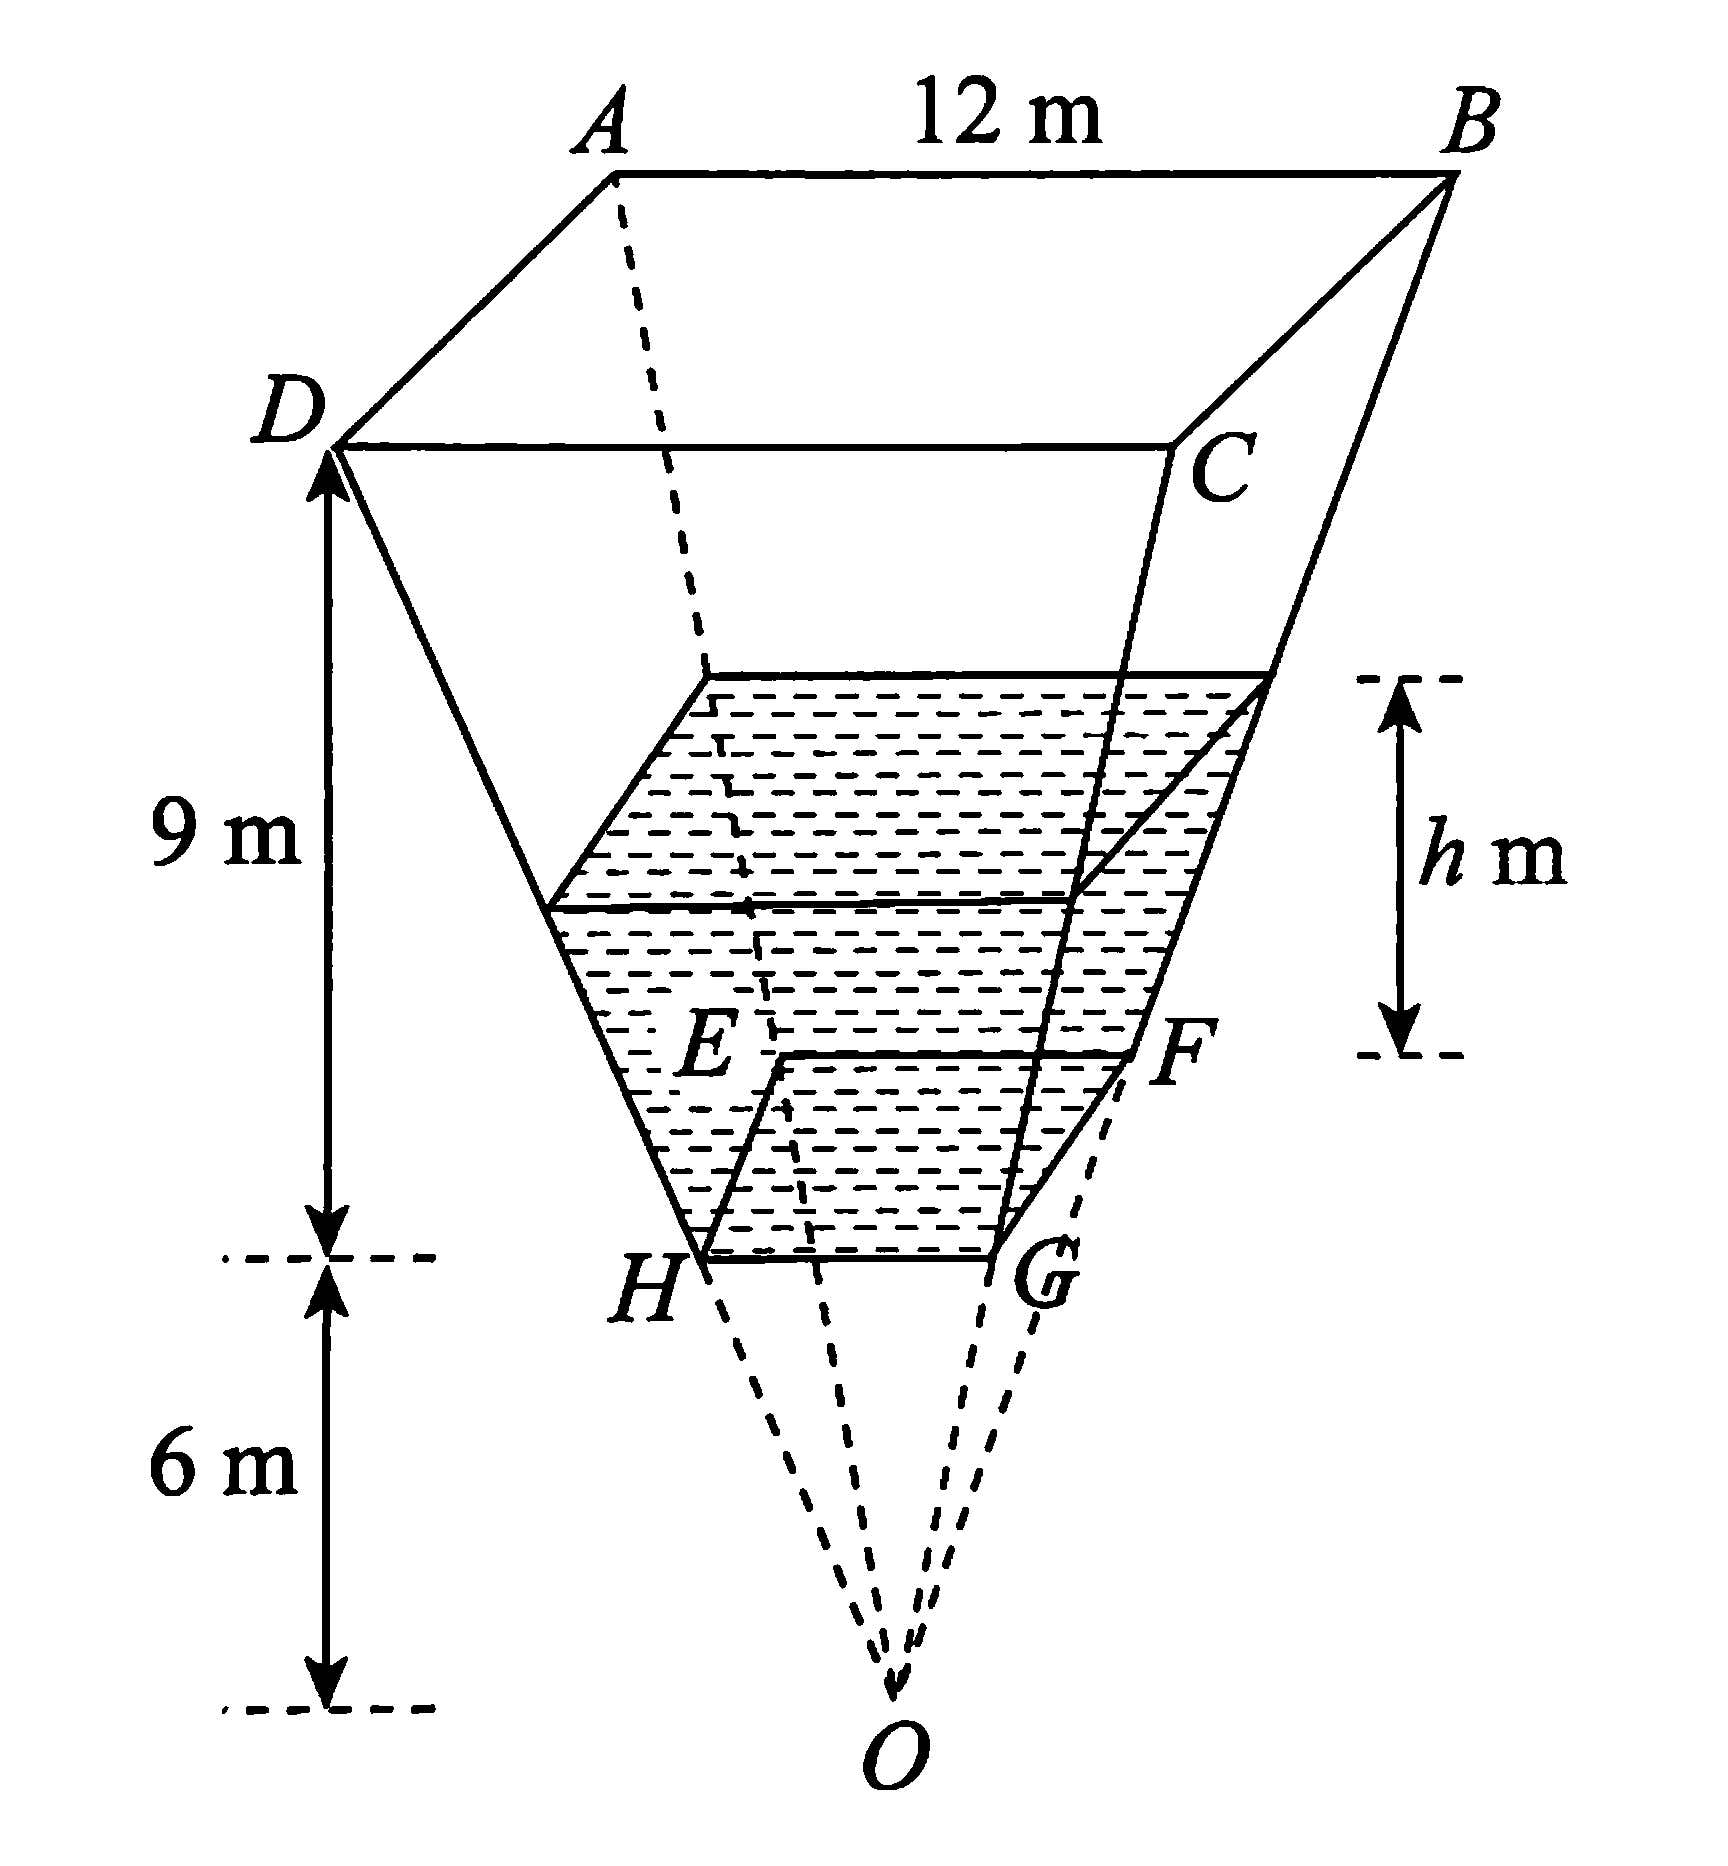
\includegraphics[scale=0.1]{./assets/download_resize_jpg.jpg}
          \end{center}

          The complete pyramid $OABCD$ has a square base of sides 12m and height 15m. THe
          depth of the tank is 9m. Water is pumped into the tan at the constant rate of
          $\dfrac{1}{3}$m$^3$min$^{-1}$.
          \begin{enumerate}
              \item Show that the volume of water $V$m$^3$ when the depth of water int he tank is
                    $h$m is given by $V = \dfrac{16}{75}h(h^2 + 18h + 108)$. \sol{}

                    Let $M$ be the midpoint of $DC$, $M'$ be the midpoint of $HG$.
                    \begin{flalign*}
                        \because   \ \triangle HOM'   & \sim \triangle DOM                             \\
                        \therefore  \ \dfrac{HM'}{DM} & = \dfrac{OM'}{OM}                              \\
                        \dfrac{HM'}{6}                & = \dfrac{6}{15}                                \\
                        HM'                           & = \dfrac{36}{15}                               \\
                        HG                            & = 2HM' = \dfrac{72}{15} = \dfrac{24}{5}        \\
                        V_{OEFGH}                     & = \dfrac{1}{3} \times 6 \times \dfrac{576}{25} \\
                                                      & = \dfrac{1152}{25}
                    \end{flalign*}
                    Let the edge of the water surface above $EFGH$ be $PQRS$. Let the mid point of $RS$ be $N$.
                    \begin{flalign*}
                        \because  \ \triangle SON  & \sim \triangle DOM                                                         \\
                        \therefore\ \dfrac{SN}{DM} & = \dfrac{ON}{OM}                                                           \\
                        \dfrac{SN}{6}              & = \dfrac{6 + h}{15}                                                        \\
                        SN                         & = \dfrac{36 + 6h}{15}                                                      \\
                                                   & = \dfrac{12 + 2h}{5}                                                       \\
                        RS                         & = 2SN                                                                      \\
                                                   & = \dfrac{24 + 4h}{5}                                                       \\
                        V_{OPQRS}                  & = \dfrac{1}{3} \times (6 + h) \times \left(\dfrac{24 + 4h}{5}\right)^2     \\
                                                   & = (6 + h) \times \dfrac{576 + 192h + 16h^2}{75}                            \\
                                                   & = \dfrac{16}{75}(6 + h)(h^2 + 12h + 36)                                    \\
                                                   & = \dfrac{16}{75}(6h^2 + 72h + 216 + h^3 + 12h^2 + 36h)                     \\
                                                   & = \dfrac{16}{75}(h^3 + 18h^2 + 108h + 216)                                 \\
                        \\
                        \therefore\ V              & = V_{OPQRS} - V_{OEFGH}                                                    \\
                                                   & = \dfrac{16}{75}(h^3 + 18h^2 + 108h + 216) - \dfrac{1152}{25}              \\
                                                   & = \dfrac{16}{75}(h^3 + 18h^2 + 108h) + \dfrac{3456}{75} - \dfrac{3456}{75} \\
                                                   & = \dfrac{16}{75}(h^3 + 18h^2 + 108h)                                       \\
                                                   & = \dfrac{16}{75}h(h^2 + 18h + 108) \quad \text{(shown)} \quad \blacksquare
                    \end{flalign*}
              \item Find the rate at which the depth is increasing at the moment when the depth of
                    water is 3m. \sol{}
                    \begin{flalign*}
                        \dfrac{dV}{dt}                                        & = \dfrac{1}{3}                                      \\
                        \dfrac{dV}{dh}                                        & = \dfrac{16(3h^2 + 36h + 108)}{75}                  \\
                        \dfrac{dh}{dt}                                        & = \dfrac{dh}{dV} \cdot \dfrac{dV}{dt}               \\
                        \dfrac{dV}{dh} \cdot \dfrac{dh}{dt}                   & = \dfrac{dV}{dt}                                    \\
                        \dfrac{16(3h^2 + 36h + 108)}{75} \cdot \dfrac{dh}{dt} & = \dfrac{1}{3}                                      \\
                        \dfrac{dh}{dt}                                        & = \dfrac{1}{3}\cdot\dfrac{75}{16(3h^2 + 36h + 108)} \\
                                                                              & = \dfrac{25}{16(3h^2 + 36h + 108)}
                    \end{flalign*}
                    When $h = 3$,
                    \begin{flalign*}
                        \dfrac{dh}{dt} & = \dfrac{25}{16\left[3(3)^2 + 36(3) + 108\right]} \\
                                       & = \dfrac{25}{16(27 + 108 + 108)}                  \\
                                       & = \dfrac{25}{16(243)}                             \\
                                       & = \dfrac{25}{3888}\text{m min}^{-1}
                    \end{flalign*}
              \item Calculate the time taken to fill up the tank if initially the tank is empty.
                    \sol{}

                    When $h = 9$,
                    \begin{flalign*}
                        V              & = \dfrac{16}{75}(9)(9^2 + 18(9) + 108) \\
                                       & = 673.92\text{m}^3                     \\
                        \dfrac{dV}{dt} & = \dfrac{1}{3}                         \\
                        V              & = \int \dfrac{1}{3}dt                  \\
                                       & = \dfrac{t}{3} + C                     \\
                    \end{flalign*}
                    When $t = 0$, $V = 0$,
                    \begin{flalign*}
                        \therefore\ C & = 0                   \\
                        V             & = \dfrac{t}{3}        \\
                        673.92        & = \dfrac{t}{3}        \\
                        t             & = 2021.76\text{ mins} \\
                                      & = 33.696\text{ hours}
                    \end{flalign*}
          \end{enumerate}
    \item Show that $\displaystyle\int_0^1 x^2\cos^{-1}xdx = \dfrac{2}{9}$. \sol{}

          Let $u = \cos^{-1}x$, $du = -\dfrac{1}{\sqrt{1 - x^2}}dx$. Let $dv = x^2dx$, $v
              = \dfrac{x^3}{3}$.
          \begin{flalign*}
              \int_0^1 x^2\cos^{-1}xdx & = \left[\dfrac{x^3}{3}\cos^{-1}x\right]_0^1 + \int_0^1 \dfrac{x^3}{3}\cdot\dfrac{1}{\sqrt{1 - x^2}}dx  \\
                                       & = \dfrac{1}{3}\cos^{-1}1 - \dfrac{0}{3}\cos^{-1}0 + \dfrac{1}{3}\int_0^1 \dfrac{x^3}{\sqrt{1 - x^2}}dx \\
                                       & = \dfrac{1}{3}\int_0^1 \dfrac{x^3}{\sqrt{1 - x^2}}dx                                                   \\
                                       & = \dfrac{1}{3}\int_0^1 \dfrac{x^2}{\sqrt{1 - x^2}}\cdot xdx
          \end{flalign*}
          Let $u = 1 - x^2$, $du = -2xdx$, $x^2 = 1 - u$.

          When x = 0, $u = 1$, when x = 1, $u = 0$.
          \begin{flalign*}
              \int_0^1 x^2\cos^{-1}xdx & = -\dfrac{1}{6}\int_1^0 \dfrac{1-u}{\sqrt{u}}du                               \\
                                       & = \dfrac{1}{6}\int_0^1 (u^{-\frac{1}{2}} - u^{\frac{1}{2}})du                 \\
                                       & = \dfrac{1}{6}\left[2u^{\frac{1}{2}} - \dfrac{2}{3}u^{\frac{3}{2}}\right]_0^1 \\
                                       & = \dfrac{1}{6}\left(2 - \dfrac{2}{3}\right)                                   \\
                                       & = \dfrac{1}{6}\cdot\dfrac{4}{3}                                               \\
                                       & = \dfrac{2}{9} \quad \text{(shown)} \quad \blacksquare
          \end{flalign*}

    \item Find the solution of the differential equation $x\dfrac{dy}{dx} - y = 2$ which
          satisfies the condition $y = 0$ when $x = 1$. \sol{} \vspace{-0.6cm}
          \begin{multicols}{2}
              \begin{flalign*}
                  x\dfrac{dy}{dx} - y                         & = 2                        \\
                  \dfrac{dy}{dx} - \dfrac{y}{x}               & = \dfrac{2}{x}             \\
                  \mu(x)                                      & = e^{\int -\dfrac{1}{x}dx} \\
                                                              & = e^{-\ln x}               \\
                                                              & = \dfrac{1}{x}             \\
                  \dfrac{1}{x}\dfrac{dy}{dx} - \dfrac{y}{x^2} & = \dfrac{2}{x^2}           \\
                  \dfrac{d}{dx}\left(\dfrac{y}{x}\right)      & = \dfrac{2}{x^2}           \\
              \end{flalign*}

              \begin{flalign*}
                  \dfrac{y}{x} & = \int \dfrac{2}{x^2}dx \\
                               & = -\dfrac{2}{x} + C     \\
                  y            & = -2 + Cx
              \end{flalign*}
              When $x = 1$, $y = 0$,
              \begin{flalign*}
                  0 & = -2 + C \\
                  C & = 2
              \end{flalign*}
              Hence, $y = 2x - 2$.
              \vfill\null
          \end{multicols}
\end{enumerate}
\end{document}